\documentclass[compress,red]{beamer}
\usepackage[utf8]{inputenc}
\usepackage{ucs}
\usepackage{amsmath}
\usepackage{amsfonts}
\usepackage{amssymb}
\usepackage[russian]{babel}
\usepackage{graphicx}
\usepackage{wrapfig}

\usepackage{tikz}
\usepackage{verbatim}

\usepackage{color}
\usepackage{xcolor}
\usepackage{listings}

\usepackage{caption}
\DeclareCaptionFont{white}{\color{white}}
\DeclareCaptionFormat{listing}{\colorbox{gray}{\parbox{\textwidth}{#1#2#3}}}
\captionsetup[lstlisting]{format=listing,labelfont=white,textfont=white}

\usetikzlibrary{calc,trees,positioning,arrows,chains,shapes.geometric,%
    decorations.pathreplacing,decorations.pathmorphing,shapes,%
    matrix,shapes.symbols}

\tikzset{
>=stealth',
  punktchain/.style={
    rectangle, 
    rounded corners, 
    % fill=black!10,
    draw=black, very thick,
    text width=10em, 
    minimum height=3em, 
    text centered, 
    on chain},
  line/.style={draw, thick, <-},
  element/.style={
    tape,
    top color=white,
    bottom color=blue!50!black!60!,
    minimum width=8em,
    draw=blue!40!black!90, very thick,
    text width=10em, 
    minimum height=1.5em, 
    text centered, 
    on chain},
  every join/.style={->, thick,shorten <=1pt},
  decoration={brace},
  tuborg/.style={decorate},
  tubnode/.style={midway, right=2pt},
}

\mode<presentation>

\usetheme{Warsaw}

\definecolor{Red}{rgb}{1,0,0}
\definecolor{Blue}{rgb}{0,0,1}
\definecolor{Green}{rgb}{0,1,0}
\definecolor{magenta}{rgb}{1,0,.6}
\definecolor{lightblue}{rgb}{0,.5,1}
\definecolor{lightpurple}{rgb}{.6,.4,1}
\definecolor{gold}{rgb}{.6,.5,0}
\definecolor{orange}{rgb}{1,0.4,0}
\definecolor{hotpink}{rgb}{1,0,0.5}
\definecolor{newcolor2}{rgb}{.5,.3,.5}
\definecolor{newcolor}{rgb}{0,.3,1}
\definecolor{newcolor3}{rgb}{1,0,.35}
\definecolor{darkgreen1}{rgb}{0, .35, 0}
\definecolor{darkgreen}{rgb}{0, .6, 0}
\definecolor{darkred}{rgb}{.75,0,0}

\xdefinecolor{olive}{cmyk}{0.64,0,0.95,0.4}
\xdefinecolor{purpleish}{cmyk}{0.75,0.75,0,0}

\useoutertheme[subsection=false]{smoothbars}


\title{Ruby: хэши}
\author{Информатика \\ 10-11 классы}

%\usecolortheme{dolphin}


\begin{document}
%%титульная страница
\maketitle
%% основные моменты

\section{Базовые сведения}

\subsection{Введение}
\begin{frame}
  \frametitle{Введение}
  \begin{itemize}
    \item Иногда возникает ситуация, когда применение массива является неудачным решением.
    \item Например, когда индексы расположены неравномерно, с большими пропусками, ведь как мы помним, ключи массива представляют собой последовательные натуральные числа + ноль.
    \item Эта проблема решается \emph{хэшами}.
    \item \emph{Хэш} --- это массив, ключами которого могут являться строки.
  \end{itemize}
\end{frame}

\subsection{Хэш vs Массив}
\begin{frame}
  \frametitle{Хэши и массивы}
	\centerline{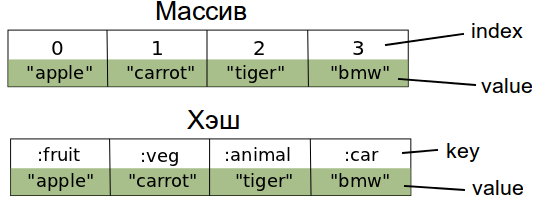
\includegraphics[width=0.9\textwidth]{images/hash_vs_array.png}}
\end{frame}

\begin{frame}[fragile]
  \frametitle{Табличная форма}
  \begin{columns}[lc]
  \column{1.2in}
    \begin{tabular}{|c|c|}
    \hline
    Ключ & Значение\\
    \hline
    ``kolya'' & 4\\
    \hline
    ``petya'' & 5\\
    \hline
    ``sergey'' & 5\\
    \hline
    ``mamba'' & 2\\
    \hline
    \end{tabular}
    
  \column{2.8in}
    \begin{itemize}
      \item Рассмотрим хэш с оценками.
      \item В ruby такой хэш записывается следующим образом:
    \end{itemize}
      \scriptsize{
      \begin{lstlisting}[language=ruby,basicstyle=\footnotesize,label=ruby1,caption=Создание хэша]
        hash = { "kolya"  => 4, 
                 "petya"  => 5, 
                 "sergey" => 5, 
                 "mamba"  => 2 } 
      \end{lstlisting}
      }
    \begin{itemize}
      \item где \rm{hash} --- название массива.
      \item Чтобы вывести на экран, например, оценку Коли, достаточно написать 
      \item \textbf{puts hash["kolya"]}.
    \end{itemize}
  \end{columns}
\end{frame}

\subsection{Создание хэша}
\begin{frame}[fragile]
  \frametitle{Создание хэша}
  
  \begin{itemize}
    \item Зададим тестовый хэш телефонных кодов стран.
  \end{itemize}
    \begin{lstlisting}[language=ruby,basicstyle=\footnotesize,label=ruby2,caption=Способы создания хэша]
    hash = { "Russia" => 7, "USA" => 1, "UK" => 44}
    
    hash = Hash.new (or hash = {})
    hash["Russia"] = 7
    hash["USA"] = 1
    hash["UK"]  = 44
    ...
    
    \end{lstlisting}

  \begin{itemize}
    \item 1 способ --- обычный, 2 --- ручной.
  \end{itemize}
  
\end{frame}

\section{Основные методы}

\subsection{Базовые методы}
\begin{frame}[fragile]
  \frametitle{Методы работы с хэшем}
    \scriptsize{
  	  Рассмотрим хэш hash = \{ ``vasya'' => 5, ``kolya'' => 4, ``petya'' => 4 \}.
		}
		\newline
		
		\scriptsize{
		\begin{tabular}{|l|l|c|}
		\hline
		\centering{\textbf{Метод}} & \centering{\textbf{Описание}} & \textbf{Результат}\\
		\hline
		hash.size & количество пар & 3 \\
		          & ``ключ-значение'' & \\
		\hline
		hash.keys & массив ключей* & [``vasya'', ``kolya'', ``petya''] \\
		\hline
		hash.values & массив значений* & [5, 4, 4] \\
		\hline
		hash.invert & поменять ключи и значения & \{5 => ``vasya'', 4 => ``kolya''\} \\
		            & местами** & \\
		\hline
		hash.max & поиск максимальной пары & [``vasya'', 5] \\
		\hline
		hash.min & поиск минимальной пары & [``kolya'', 4] \\
		\hline
		hash.delete(``vasya'') & удалить элемент по ключу & \{ ``kolya'' => 4, ``petya'' => 4 \} \\
		\hline
		\end{tabular} }
		
		* хэши в ruby неупорядочены: массивы могут иметь любой порядок элементов.
		** при ``перевороте'' в случае совпадения значений будет выбрано первое.
\end{frame}

\subsection{Методы работы}
\begin{frame}[fragile]
  \frametitle{Методы работы с хэшем - 2}
    \scriptsize{
  	  Рассмотрим хэш hash = \{ ``vasya'' => 5, ``kolya'' => 4, ``petya'' => 4 \}.
		}
		\newline
		
		\scriptsize{
		\begin{tabular}{|l|l|c|}
		\hline
		\centering{\textbf{Метод}} & \centering{\textbf{Описание}} & \textbf{Результат}\\
		\hline
		hash.empty? & есть ли хоть один элемент & false \\
		\hline
		hash.key?(``vasya'') & есть ли в хэше элемент & true \\
		                     & с ключом vasya         &      \\
 		\hline
 		hash.has\_key?(``vasya'') & аналогично & true \\
 		\hline
 		hash.include?(``vasya'') & аналогично & true \\
		\hline
		hash.value?(3) & есть ли в хэше элемент & false \\
                    & со значением 3         &       \\
		\hline
 		hash.has\_value?(3) & аналогично & false \\
		\hline
		\end{tabular}}
\end{frame}

\section{Сортировка и экстремумы}
\subsection{Сортировка}
\begin{frame}[fragile]
  \frametitle{Сортировка по ключу}

  \begin{itemize}
    \item Как и массивы, хэши можно сортировать с помощью метода \textbf{sort}.
    \item Однако на выходе получается не хэш, а двумерный массив пар ``ключ-значение''.
    \item Базово сортировка проводится \textbf{по ключам}, а не по значениям, как в массивах.
  \end{itemize}

  \scriptsize{
    \begin{lstlisting}[language=ruby,basicstyle=\footnotesize,label=ruby4,caption=Сортировка по ключам]
      hash = { "abc" => 10, "def" => 7, "aac" => 25}
      hash_sorted = hash.sort
      puts hash_sorted.inspect 
      # [["aac", 25], ["abc", 10], ["def", 7]]
    \end{lstlisting}
  }
\end{frame}

\subsection{Сортировка по значению}
\begin{frame}[fragile]
  \frametitle{Сортировка по значению}

  \begin{itemize}
    \item Для сортировки по значению есть специальный метод \emph{sort\_by}.
    \item На выходе опять получается не хэш, а двумерный массив пар ``ключ-значение''.
  \end{itemize}

  \scriptsize{
    \begin{lstlisting}[language=ruby,basicstyle=\footnotesize,label=ruby5,caption=Сортировка по ключам]
      hash = { "abc" => 10, "def" => 7, "aac" => 25}
      hash_sorted = hash.sort_by { |key, value| value }
      puts hash_sorted.inspect 
      # [["def", 7], ["abc", 10], ["aac", 25]]
    \end{lstlisting}
  }
  
\end{frame}

\subsection{Максимальный и минимальный элементы}
\begin{frame}[fragile]
  \frametitle{Максимальный и минимальный элементы}

  \begin{itemize}
    \item Максимальный и минимальный элементы хэша можно найти с помощью методов \textbf{max}, \textbf{min}, \textbf{max\_by}, \textbf{min\_by}.
    \item На выходе --- массив из двух элементов (ключ и значение). 
    \item Первые два метода ищут экстремум по ключу, вторые два --- по условию.
  \end{itemize}

  \scriptsize{
    \begin{lstlisting}[language=ruby,basicstyle=\footnotesize,label=ruby6,caption=Максимальный и минимальный элементы]
      hash = { "abc" => 10, "def" => 7, "aac" => 25}
      puts hash.max # ["def", 7]
      puts hash.min # ["aac", 25]
      puts hash.max_by{ |key, value| value } # ["aac", 25]
      arr = hash.min_by{ |key, value| value } 
      puts arr # ["def", 7]
    \end{lstlisting}
  }
\end{frame}

\subsection{Преобразование хэша в массив}
\begin{frame}[fragile]
  \frametitle{Преобразование хэша в массив}

  \begin{itemize}
    \item Иногда в целях удобства (или исходя из технических особенностей, как в методах \textbf{sort\_by} и пр.) хэши преобразуют в двумерный массив пар ``ключ--значение''.
    \item Для преобразования используется метод \textbf{to\_a}.
  \end{itemize}

  \scriptsize{
    \begin{lstlisting}[language=ruby,basicstyle=\footnotesize,label=ruby7,caption=Преобразование в массив]
      hash = { "abc" => 10, "def" => 7, "aac" => 25}
      arr  = hash.to_a
    \end{lstlisting}
  }

  \begin{itemize}
    \item В итоге в массив arr будет следующим: [ [``abd'', 10], [``def'', 7], [``aac'', 25] ]
  \end{itemize}
  
\end{frame}

\section{Итераторы}
\subsection{Итераторы}
\begin{frame}[fragile]
  \frametitle{Итераторы}

  \begin{itemize}
    \item Аналогично массивам для хэшей можно использовать методы \textbf{map}, \textbf{find\_all}, \textbf{inject}.
    \item В качестве параметра--``ключа'' внутри цикла появляется не просто обычная переменная, а массив из двух элементов --- ключа и значения!
  \end{itemize}

  \scriptsize{
    \begin{lstlisting}[language=ruby,basicstyle=\footnotesize,label=ruby8,caption=Итераторы]
      hash = { "abc" => 10, "def" => 7, "aac" => 25}
      res1 = hash.find_all{|array| array[1] < 20} 
      res2 = hash.map { |array| array[1]*2 }
      res3 = hash.inject(0){ |res, arr| res+arr[1] }
    \end{lstlisting}
  }

  \begin{itemize}
    \item Что будет в каждой из переменных?
  \end{itemize}

\end{frame}

\subsection{Результаты итераторв}
\begin{frame}
  \frametitle{Результаты работы итераторов}
  \begin{itemize}
    \item В переменной \textbf{res1} окажется двумерный массив элементов, чьи значения меньше 20: [[``abc'', 10], [``def'', 7]]. Обратите внимание, что результатом вновь окажется именно массив, а не хэш.
    \item В переменной \textbf{res2} окажется одномерный массив значений, умноженных на 2: [20, 50, 14].
    \item В переменной \textbf{res3} будет находиться сумма всех значений хэша: 42.
    \item \textbf{NB}: Не забывайте, что переменная--ключ, используемая в итератора, в случае хэша является массивом из двух элементов --- ключа и значения!
  \end{itemize}
\end{frame}

\subsection{Альтернативная запись итераторов}
\begin{frame}[fragile]
  \frametitle{Альтернативная запись итераторов}

  \begin{itemize}
    \item Если массивы внутри итератора вызывают эстетическое отвращение, можно записать в виде переменных.
    \item Напишем ту же самую программу, но в другой форме.
    \item Обратите особое внимание на метод inject. Скобочки там стоят не для красоты!
  \end{itemize}

  \scriptsize{
    \begin{lstlisting}[language=ruby,basicstyle=\footnotesize,label=ruby9,caption=Альтернативная запись]
      hash = { "abc" => 10, "def" => 7, "aac" => 25}
      res1 = hash.find_all{|key, value| value < 20} 
      res2 = hash.map { |key, value| value*2 }
      res3 = hash.inject(0){ |res, (key, value)| res+value }
    \end{lstlisting}
  }

\end{frame}

\subsection{Повторяемость в массиве}
\begin{frame}[fragile]
  \frametitle{Сумма}
		\begin{itemize}
  		\item Допустим даны оценки Васи: arr = [3, 5, 5, 4, 5, 2].
  		\item Определим, сколько раз и какую Оценку Вася получил.
  	\end{itemize}
  	\scriptsize{
  		\begin{lstlisting}[language=ruby,basicstyle=\footnotesize,label=ruby3,caption=Повторяемость]
  		  arr = [3, 5, 5, 4, 5, 2]
  		  marks = arr.inject(Hash.new{ 0 }){ |res, elem| 
  		    res[elem] += 1
  		    res
  		  }
  		  puts marks.inspect
      \end{lstlisting}}
\end{frame}

\subsection{Inject}
\begin{frame}[fragile]
  \frametitle{Разбор программы}

  \begin{itemize}
    \item В данном примере мы используем развёрнутую нотацию метода inject.
    \item Конструкция \textbf{Hash.new\{ 0 \}} означает: создать пустой хэш и сделать любой несуществующий элемент по умолчанию равным нулю.
    \item \textbf{Алгоритм}: заведём хэш res, в котором ключами будут оценки, а значениями --- их количество. Изначально каждой оценки --- 0 штук.
    \item Пробегаем по всему массиву \textbf{arr}. Берём пробегаемую оценку и увеличиваем количество этих оценок в хэше res на 1. 
    \item Результат выполнения inject записываем в хэш marks.
    \item Для полного вывода на экран переменной используем специальный метод \textbf{inspect}.
  \end{itemize}
  
\end{frame}
\subsection{Из массива в хэш}
\begin{frame}[fragile]
  \frametitle{Из массива в хэш}

  \begin{itemize}
    \item Как преобразовать массив в хэш?
    \item Пусть дан массив arr. Как сделать чётные элементы ключами хэша, а нечётные --- значениями?
  \end{itemize}

  \scriptsize{
    \begin{lstlisting}[language=ruby,basicstyle=\footnotesize,label=ruby10,caption=Из массива в хэш]
      arr  = [ "abc", 10, "def", 7]
      hash = Hash[*arr] 
      puts hash.inspect
      # {"abc"=>10, "def"=>7}
    \end{lstlisting}
  }

\end{frame}
\subsection{Из массива в хэш 2}
\begin{frame}[fragile]
  \frametitle{Из двумерного массива в хэш}

  \begin{itemize}
    \item А если массив двумерный?
    \item Пусть дан двумерный массив ``ключ--значение'' arr.
    \item Сделаем из него хэш. Для этого сначала ``сплющим'' массив методом \textbf{flatten}.
  \end{itemize}

  \scriptsize{
    \begin{lstlisting}[language=ruby,basicstyle=\footnotesize,label=ruby11,caption=Из массива в хэш]
      arr  = [ ["abc", 10], ["def", 7]]
      hash = Hash[*arr.flatten] 
      puts hash.inspect
      # {"abc"=>10, "def"=>7}
    \end{lstlisting}
  }

\end{frame}

\section{Задания}
\subsection{Задания 1}
\begin{frame}
  \frametitle{Задания}
  \begin{itemize}
    \item Дана строка s. Посчитать, сколько раз какое слово там встречается?
    \item Предыдущая задача, только вывести ТОП-10 часто встречающихся слов в порядке убывания.
  \end{itemize}
\end{frame}

\subsection{Задания 2}
\begin{frame}
  \frametitle{Задания}
  \begin{itemize}
    \item Дан массив строк arr. Каждая строка содержит информацию в следующем формате: дата (число из двух цифр, затем символ ТОЧКА, затем месяц из двух цифр. Примеры: 13.02, 01.01), символ ПРОБЕЛ, температура в виде вещественного числа. Пример правильно оформленной строки (одной из многих в массиве): ``02.11 -3.2''. Необходимо сосчитать среднемесячную температуру на каждый месяц, исходя из представленных данных и вывести её на экран по месяцам, начиная с января. Если на какой-либо месяц данные отсутствуют, то напротив этого месяца вывести словосочетание ``данные отсутствуют''.
  \end{itemize}
\end{frame}

\subsection{Задания 3}
\begin{frame}
  \frametitle{Задания}
  \begin{itemize}
    \item Дан двумерный массив, состоящий из двух одномерных массивов равной длины. Составить из этого массива хэш, ключами которого являются элементы первого подмассива, а значениями --- второго. Пример: arr = [ [1,2,3], [4,5,6] ]. Из этого массива должен получиться хэш hash = \{ 1 => 4, 2 => 5, 3 => 6 \}.
    \item Дан кусок текста в виде строковой переменной s. Посчитайте количество 10 любых союзов (например, ``а'', ``и'', ``а то'' и пр.) и выведите их в порядке встречаемости в тексте, начиная с самого часто встречающегося.
    \item Найти самое употребляемое слово во Вступлении к поэме А.С. Пушкина ``Медный всадник''.
  \end{itemize}
\end{frame}

\section{References}
\subsection{References}
\begin{frame}[fragile]
  \frametitle{References}
  \begin{itemize}
    \item При подготовке данного материала использовались сайты: http://ru.wikibooks.org/wiki/Ruby, http://rubydev.ru, http://en.wikipedia.org, http://ruby-lang.org.
    \item Все презентации доступны на http://school.smirik.ru!
    \item Вопросы, предложения, д/з: smirik@gmail.com
  \end{itemize}
\end{frame}

\end{document}